\documentclass{article}


\usepackage{siunitx} % Provides the \SI{}{} and \si{} command for typesetting SI units
\usepackage{graphicx} % Required for the inclusion of images
\usepackage{natbib} % Required to change bibliography style to APA
\usepackage{amsmath} % Required for some math elements 
\usepackage{listings}
\usepackage{placeins}
\usepackage{color}
\setlength\parindent{0pt} % Removes all indentation from paragraphs

\lstset{frame=tb,
  language=Matlab,
  aboveskip=3mm,
  belowskip=3mm,
  showstringspaces=false,
  columns=flexible,
  basicstyle={\small\ttfamily},
  numbers=none,
  numberstyle=\tiny\color{gray},
  keywordstyle=\color{blue},
  commentstyle=\color{green},
  stringstyle=\color{red},
  breaklines=true,
  breakatwhitespace=true,
  tabsize=3}
%\renewcommand{\labelenumi}{\alph{enumi}.} % Make numbering in the enumerate environment by letter rather than number (e.g. section 6)


\title{Lab 2 \\ Analyzing Sinusoids with Varying Frequency and Convolution in Smoothing} % Title

\author{Aneesh Malhotra \\ G00844135} % Author name

\date{\today} % Date for the report

\begin{document}

\maketitle % Insert the title, author and date


% If you wish to include an abstract, uncomment the lines below
% \begin{abstract}
% Abstract text
% \end{abstract}

%----------------------------------------------------------------------------------------
%	SECTION 1
%----------------------------------------------------------------------------------------

\section{Introduction}



% If you have more than one objective, uncomment the below:
\begin{description}
\item[First Objective] \hfill \\
The first objective of this lab was to analyze sinusoids with varying instantaneous frequency. This was done by creating a function $\theta(t)$ such that $\frac{d \theta}{dt} = \omega(t)$. Using this we created signals that varied in frequency both linearly and quadratically, and confirmed our results using a spectrogram.
\item[Second Objective] \hfill \\
The second goal of this lab was to analyze how the convolution operation can smooth out signals. We started with a simple DC signal and saw how through several convolutions the signal became closer to a Gaussian distribution, a smooth function. We did this again with a noise signal and obtained the same results.
\end{description}

%----------------------------------------------------------------------------------------
%	SECTION 2
%----------------------------------------------------------------------------------------

\section{Main Body}

\subsection{Constant Signal}


We began by defining our sample frequency as $f_s = 14400$ and our fundamental frequency $f_0 = 440.$ Our time vector $t$ consisted of time samples at the sample period $T_s = \frac{1}{f_s}$ on the interval $[0,1]$. We obtained the following plot of the first 200 samples of a sinusoid with frequency $f_0$.
\begin{figure}
	\centering
		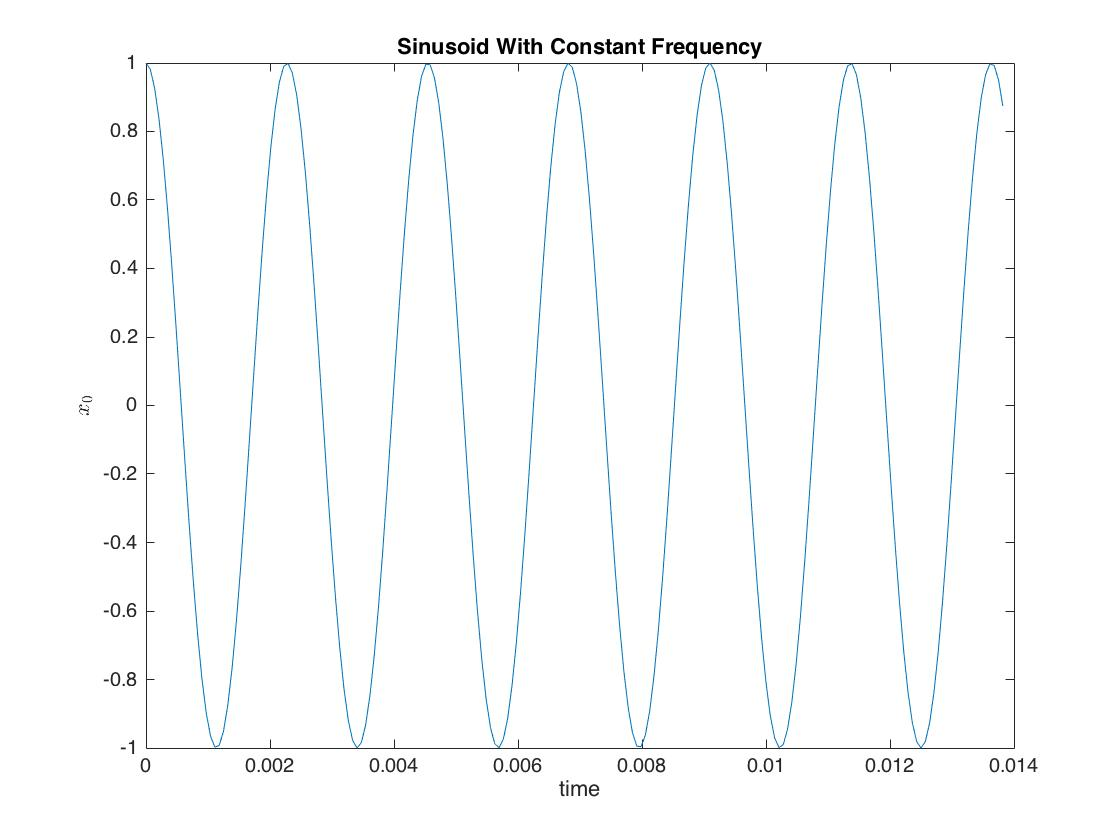
\includegraphics[width =0.8\linewidth, height = 0.3\textheight]{part2x0.jpg}
	\caption{First 200 Samples of $\cos(2 \pi 440 t)$}
\end{figure}

\FloatBarrier
\subsection {Frequency-Varying Signals}
Next we created signals with varying frequency. In order to do this, we needed to identify a function $\theta(t)$ such that its derivative is the desired function of angular frequency. We initially created a signal that starts at $4400 \si{Hz}$ and ends at $5500 \si{Hz}$ in the duration of one second. In order to do this, we calculate the the angular frequency function $\omega(t)$. 
\begin{align*}
\frac{\Delta y}{\Delta t} &= \frac{5500 - 4400}{1} = 1100 \\
\omega(t) &= 2\pi(4400 + 1100t)
\end{align*}

Now that we have $\omega(t)$ we can integrate to obtain $\theta(\tau)$.

$$ \theta(t) = 2\pi \int_{0}^{t} 4400 + 1100\tau  \,d \tau.$$ Therefore
$$\theta(t) = 2 \pi (440t + 1100 \frac{t^2}{2}).$$

This calculation was repeated for signals with linearly decreasing, triangular, and quadratically increasing frequencies. We obtained the following spectrograms:

\begin{figure}[!htb]
    \centering
    \begin{minipage}{.5\textwidth}
        \centering
        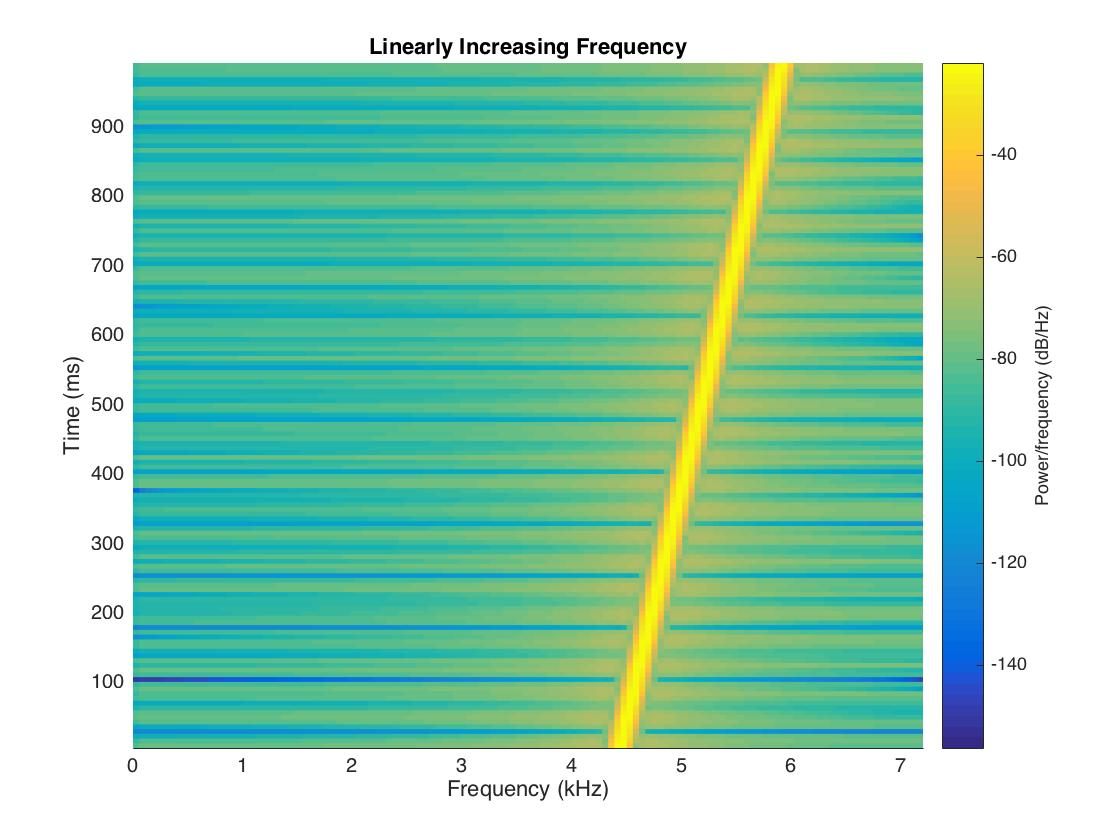
\includegraphics[width=1.0\linewidth, height=0.2\textheight]{part2li.jpg}

        \label{fig:prob1_6_2}
    \end{minipage}%
    \begin{minipage}{0.5\textwidth}
        \centering
        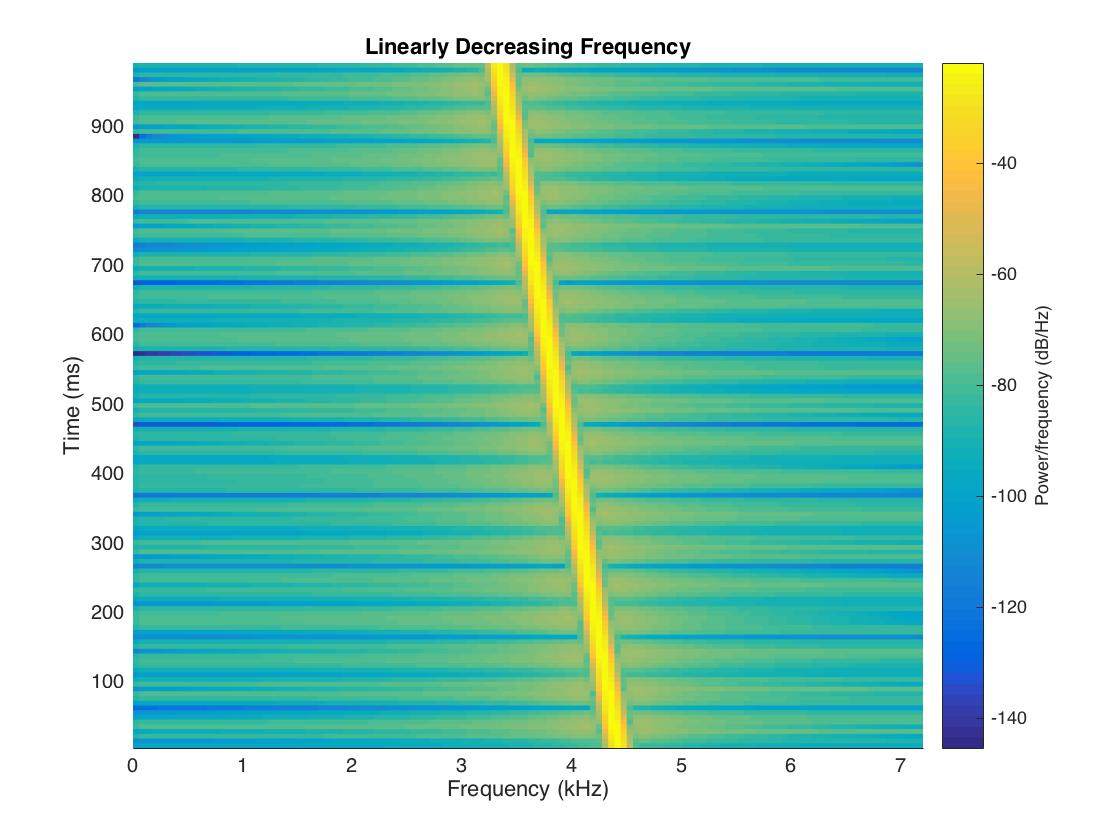
\includegraphics[width=1\linewidth, height=0.2\textheight]{part2ld.jpg}

        \label{fig:prob1_6_1}
    \end{minipage}
    \caption{Linearly Increasing and Decreasing Frequencies}
\end{figure}

\begin{figure}[!htb]
    \centering
    \begin{minipage}{.5\textwidth}
        \centering
        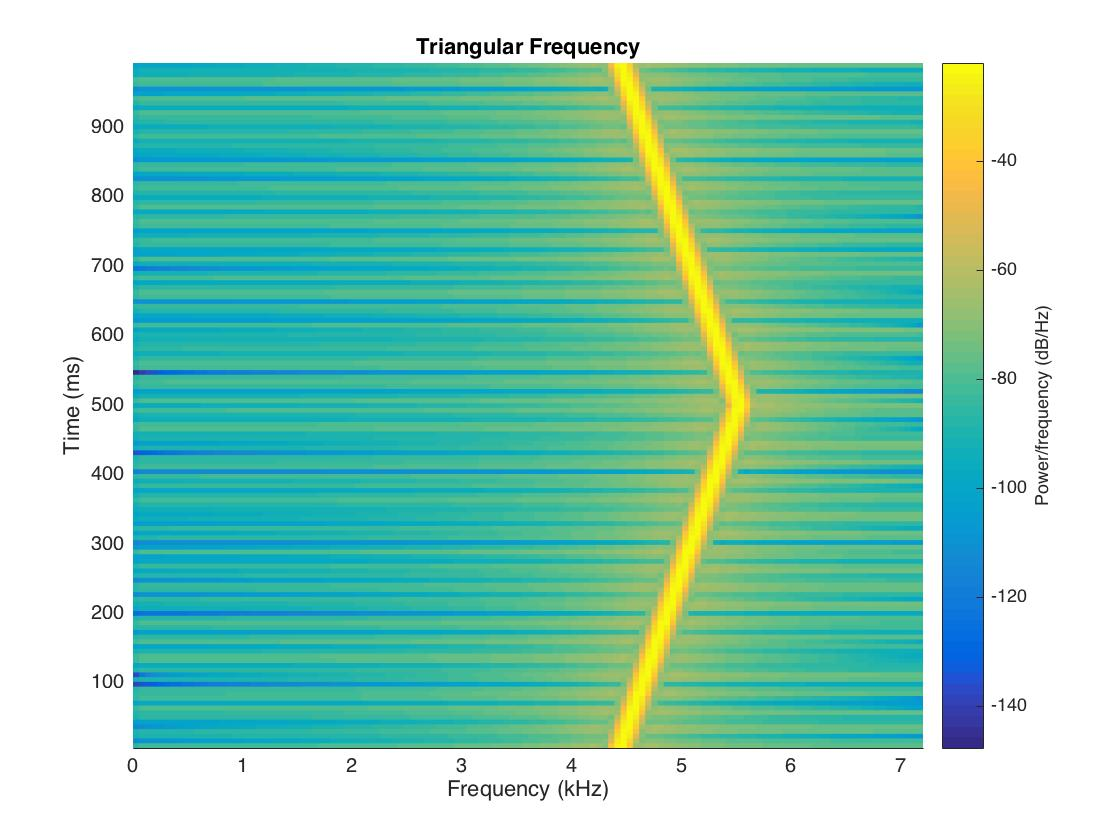
\includegraphics[width=1.0\linewidth, height=0.2\textheight]{part2triangle.jpg}

        \label{fig:prob1_6_2}
    \end{minipage}%
    \begin{minipage}{0.5\textwidth}
        \centering
        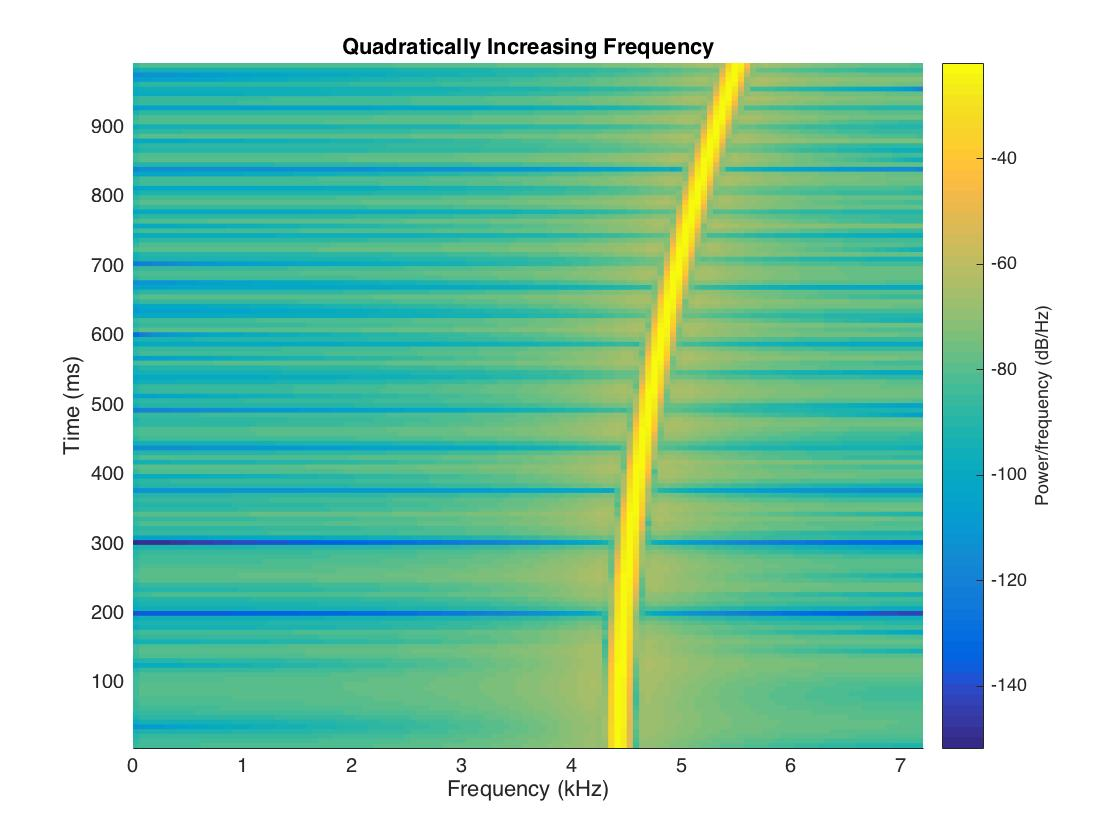
\includegraphics[width=1\linewidth, height=0.2\textheight]{part2quad.jpg}

        \label{fig:prob1_6_1}
    \end{minipage}
    \caption{Triangular and Quadratic Frequencies}
\end{figure}


\FloatBarrier
\subsection{Convolution and Smoothing}

In this section we looked at the convolution operation and how it tends to smooth functions when applied continuously. We began with a square signal $p_0 (t)$ that takes the value of $1$ when $0 \leq t \leq 1$ and is $0$ otherwise. We applied the convolution operation such that $p_1(t) = p_0(t) * p_1(t)$,  $p_2(t) = p_1(t) * p_1(t)$, and so forth. Each of the outputs was normalized by the maximum value of the signal and scaled in time so that we can analyze each signal on the same time axis.

\begin{figure}[!htb]
    \centering
        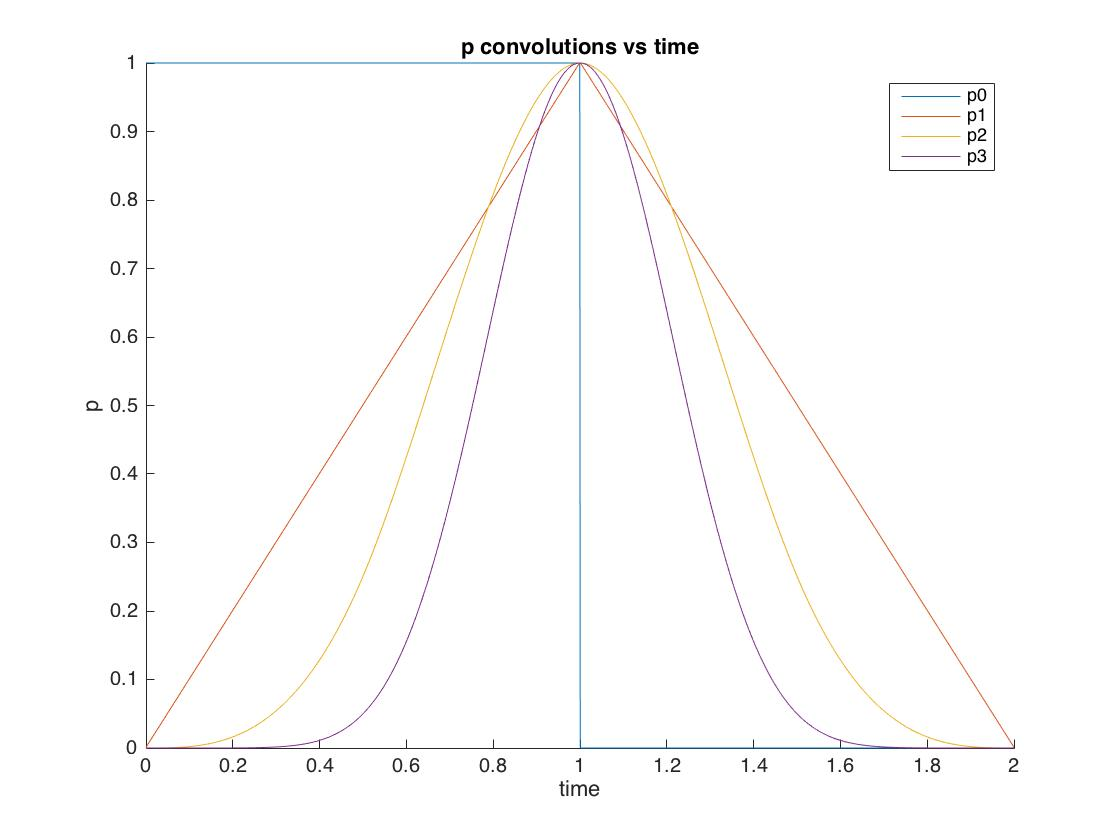
\includegraphics[scale = 0.32]{part3pplot.jpg}
        \caption{Plots of a Square Signal With Multiple Convolutions}
\end{figure}

\FloatBarrier
This was repeated for a noise signal obtained using the command rand(2000,1) and the following plot was obtained

\begin{figure}[!htb]
    \centering
        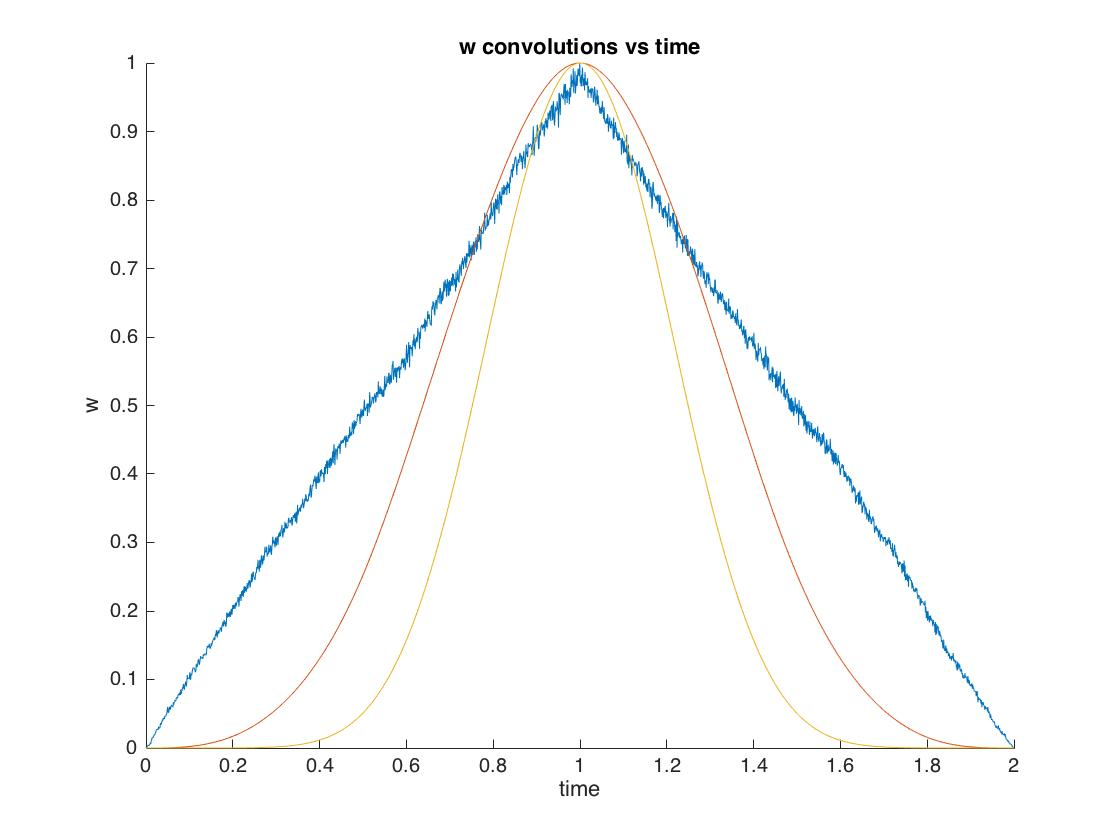
\includegraphics[scale = 0.32]{part3wplot.jpg}
        \caption{Plots of a Noise Signal With Multiple Convolutions}
\end{figure}

\FloatBarrier

We see that in both cases, the signal tends to become more bell-shaped. We confirm this by seeing the traditional bell curve given by the Gaussian function $$ g(t) = e^{-\frac{1}{2}(\frac{t-1}{a} ^2)}.$$ 

\begin{figure}[!htb]
    \centering
        \includegraphics[scale = 0.25]{Gaussian.jpg}
        \caption{Plots of a Gaussian Distribution}
\end{figure}

\begin{figure}[!htb]
    \centering
        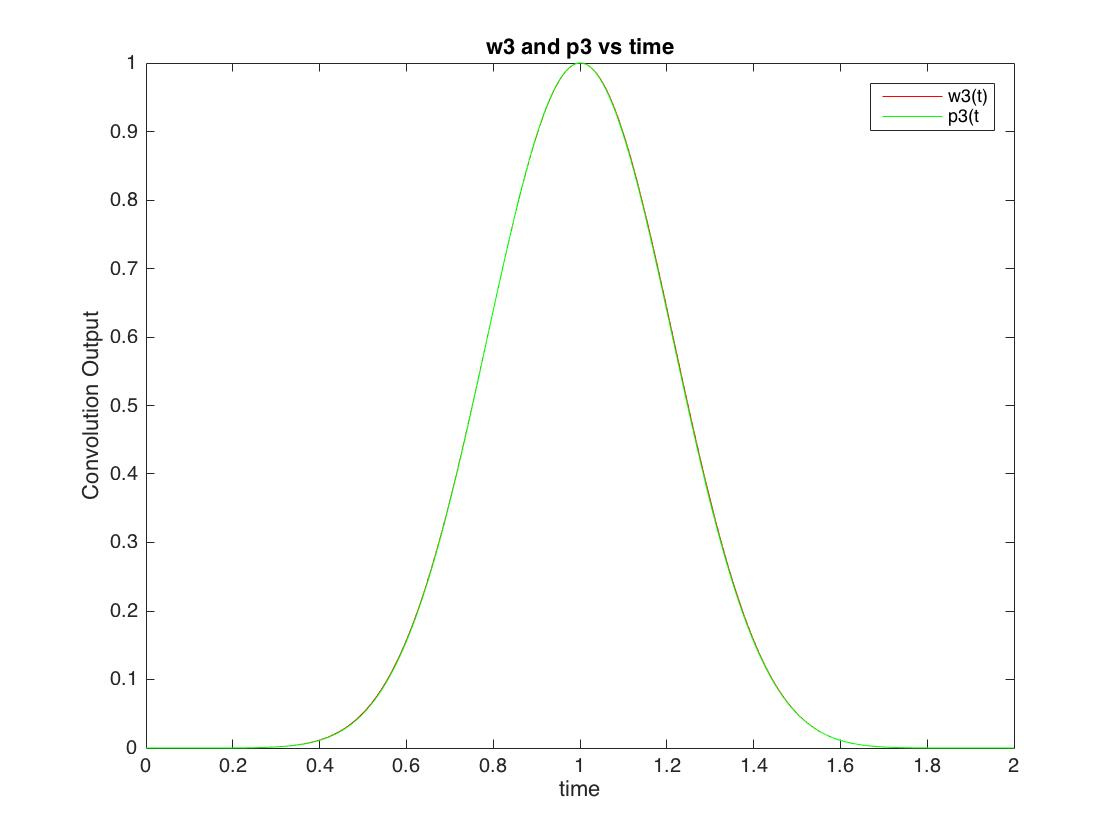
\includegraphics[scale = 0.25]{part3compare.jpg}
        \caption{Plots of $p_3$ and $w_3$ }
\end{figure}



\FloatBarrier
We see that the plot of the Gaussian distribution is very similar to those of $p_3$ and $w_3$.

%----------------------------------------------------------------------------------------
%	SECTION 4
%----------------------------------------------------------------------------------------
\FloatBarrier
\section{Conclusion}
\subsection{Sinusoids with Varying Frequency}
In this section we plotted and analyzed sinusoids whose frequencies varied with time. In order to do this we algebraically solved for a function that describes the angular frequency instantaneously in time, and integrated to find the input argument to the cosine function. I chose to integrate from a starting value of $t = 0$, although we could technically choose any constant to add, as it would only affect the phase of the signal and not the instantaneous frequency. The most difficult frequency function to plot was the triangular as it required splitting the time domain into an increasing and decreasing part and combining them (see Appendix for code). We also listened to each of these signals to see the qualitative effect of varying the frequency. As expected, the linearly increasing and decreasing signals were chirps whose pitches varied. The triangular frequency did as expected and increased in pitch and then decreased back to its original pitch. The quadratic signal was interesting as the pitch started off having a very low rate of change and obtained a higher rate in time.
\subsection{Convolution and Smoothing}
In this section we applied the convolution operation several time to both a square wave and a noise function. Both, however, resulted in a Gaussian distribution. I explain this phenomenon using probability. The expected value of the sum of two probability density functions is the convolution between them. By the central limit theorem, if we look at each distribution as an experiment, the sum of the data should approach a Gaussian distribution. This is what we saw with these signals. Both signals started off as being very sharp, and contained discontinuities, but approach a Gaussian when applied to an LTI system. This is interesting because we are taking a function with discontinuities and making it continuously differentiable for all values in the domain. 
\section{Appendix}

\subsection{Part 2 Code}
\lstinputlisting{lab_022.m}
\subsection{Part 3 Code}
\lstinputlisting{lab_023.m}


%----------------------------------------------------------------------------------------
%	BIBLIOGRAPHY
%----------------------------------------------------------------------------------------
\section{References}

Lathi, B. P. Linear Systems and Signals. New York: Oxford UP, 2005. Print.

\end{document}